\chapter{Numerical Time Integration of Partial/Ordinary Differential Equations}

\section{Introduction}

Many engineering problems are described as either a partial differential equation (PDE) or ordinary differential equation (ODE). A broad class of important problems is called the ``Initial Value Problem'' (IVP). Take for example the continuity equation in semiconductors, which is given as\begin{IEEEeqnarray}{rCl}
\frac{\partial n}{\partial t} & = & -\text{div}\left(\bm{J}\right) + G_\text{n} - R_\text{n} \label{eq:continuityEqn}
\end{IEEEeqnarray}where $n$ is the carrier concentration, $\bm{J}$ is the current density flowing through the semiconductor, $G_\text{n}$ and $R_\text{n}$ are the rates of carrier generation and recombination due to generation and recombination processes, respectively. The IVP would be as follows: assume that at time, $t=0$, the carrier concentration is $n(t=0)={0}$ and we want to find the time-dependent profile of the carrier concentration, $n(t)$.

In general, the PDE is more complicated than that in Equation~(\ref{eq:continuityEqn}), and the time derivative or slope function is denoted as $\dot{y}(t)=f(t, y)$, where $y(t)$ is the quantity we are trying to solve for, having the initial condition $y(t=0)=y_{0}$.

\section{The Forward (Explicit) Euler Method}

One method to obtain $y(t)$ from $f(t,y)$ and $y_{0}$ is to use the forward Euler method. First, the time range over which to determine $y(t)$ is discretized into a uniform grid. The time difference between each grid point, $\Delta t=h$ is called the \emph{time step}. $y(t)$ is then iteratively calculated (starting at $y_{0}$) using the formula\begin{IEEEeqnarray}{rCl}
y(t+h) & = & y(t) + hf(t,y(t)) \label{eq:compExEuler}
\end{IEEEeqnarray}Mathematically, the Equation~(\ref{eq:compExEuler}) is unwieldy and we simplify the expression using $y_{n+1}=y(t+h)$ and $y_{n}=y(t)$, which gives\begin{IEEEeqnarray}{rCl}
y_{n+1} & = & y_{n} + hf(t,y_{n}) \label{eq:simpExEuler}
\end{IEEEeqnarray}

\subsection{Example 1}

Consider the function $y(t) = \sin (t)$ and its time derivative, $\dot{y}(t) = \cos (t)$. The numerical solution for different time steps are plotted in Fig.~\ref{fig:IVP1}.
\begin{figure}[!b]
\centering
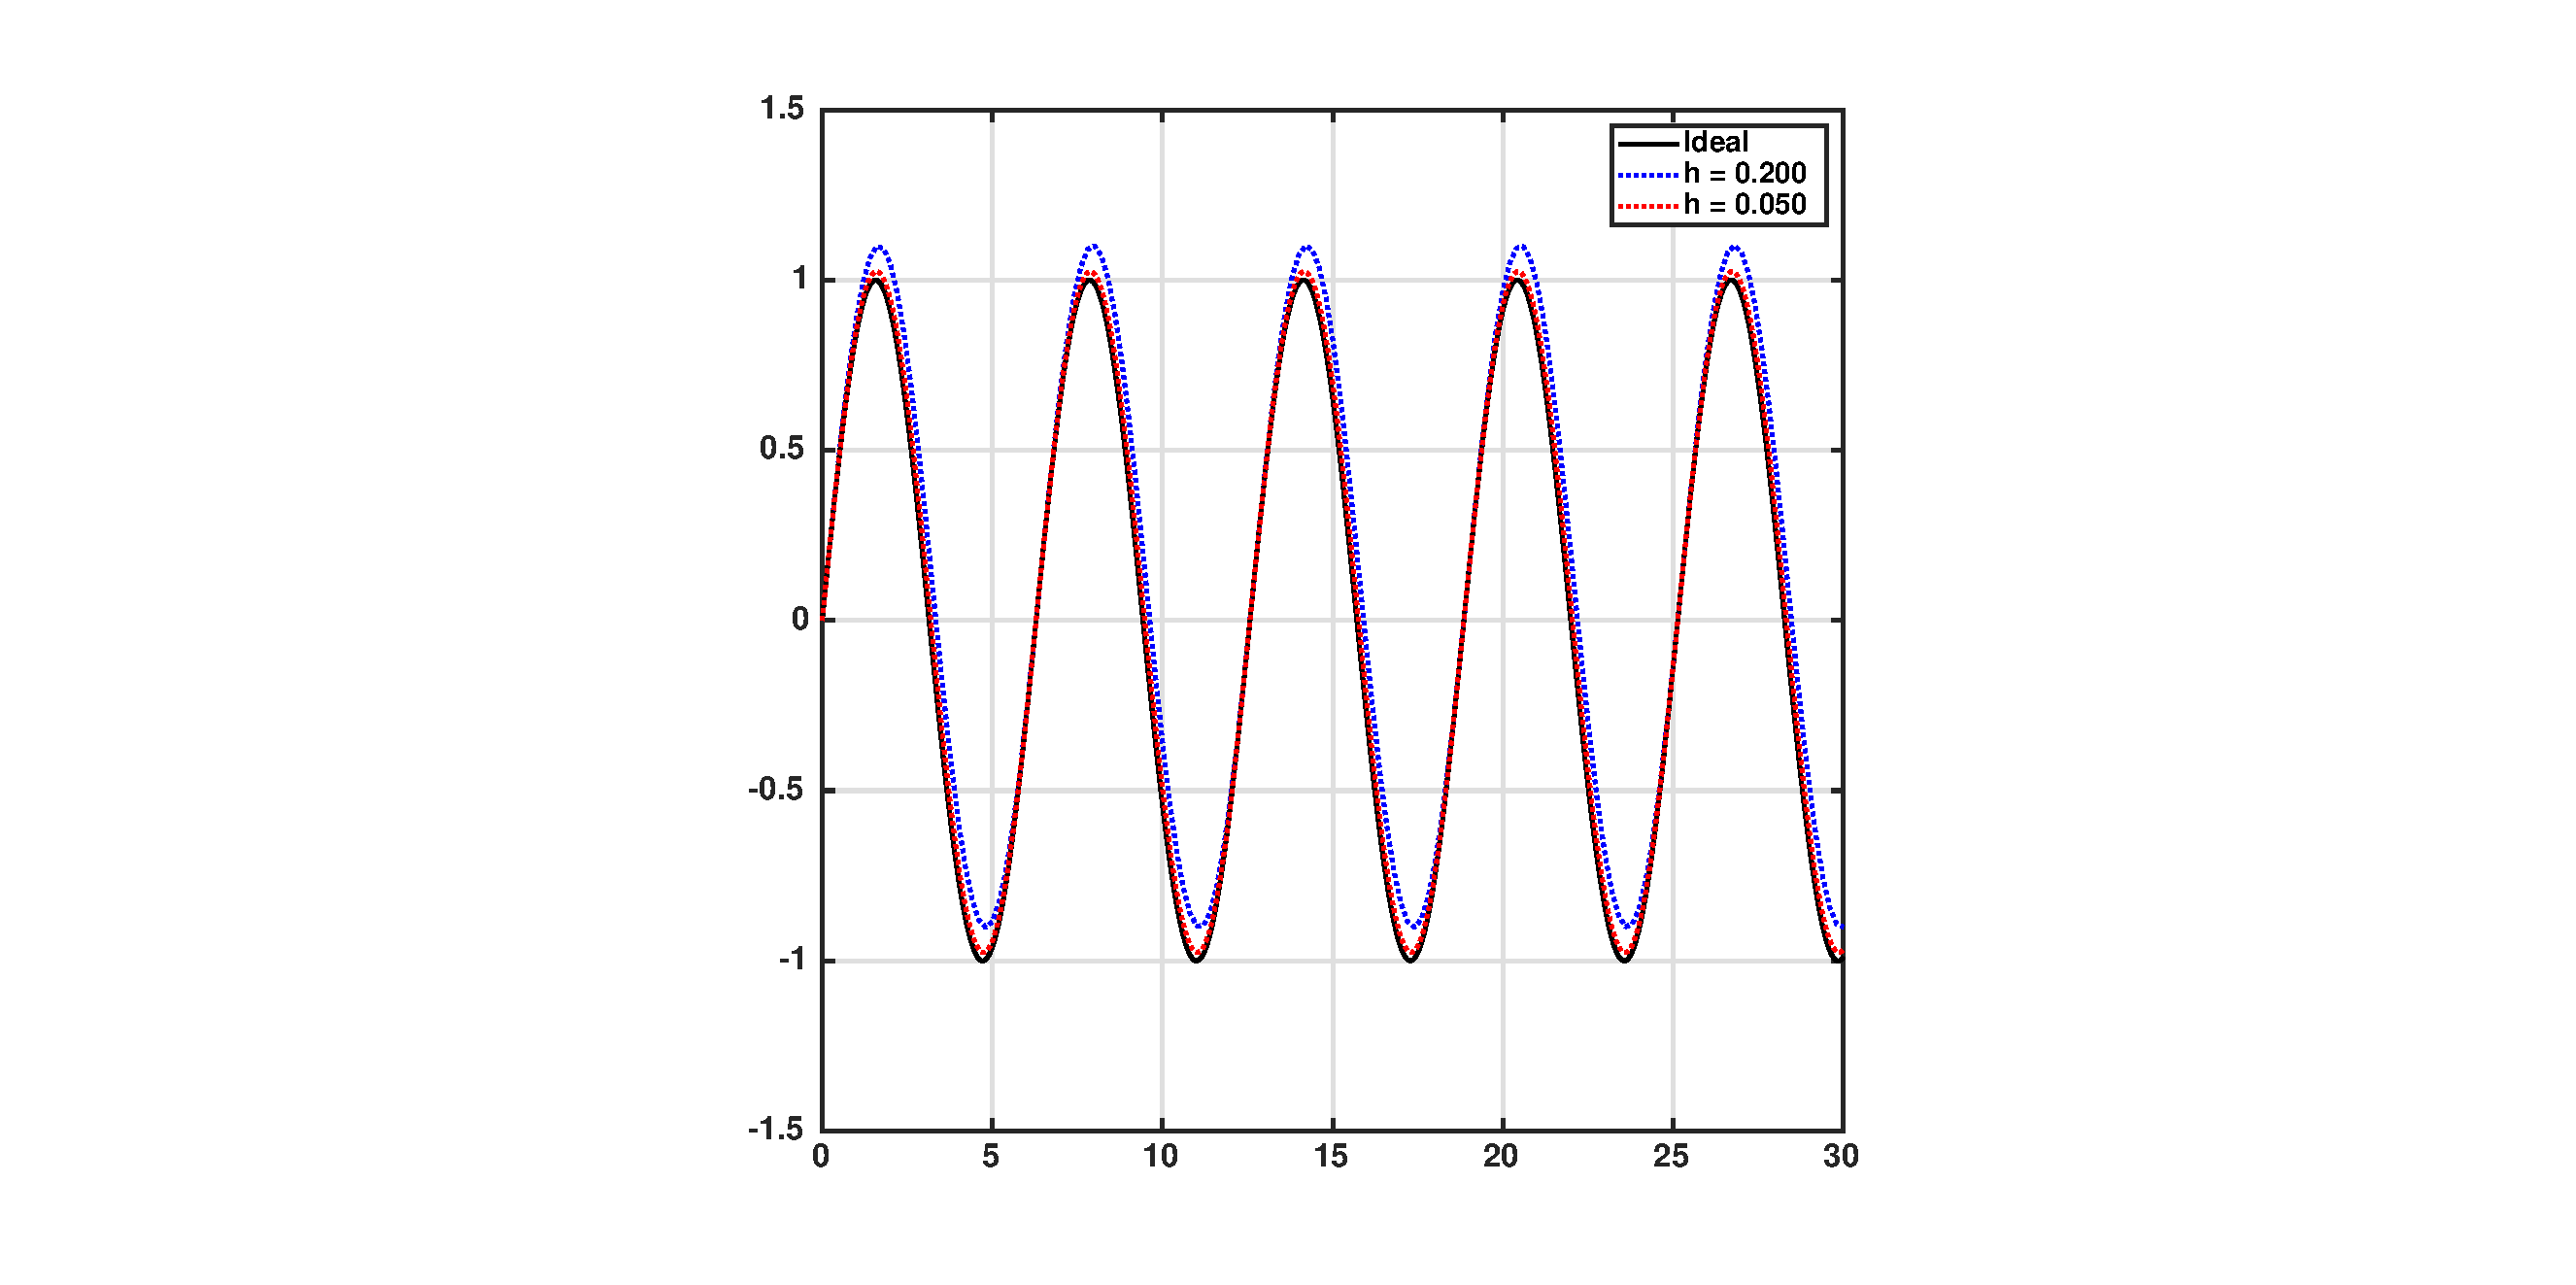
\includegraphics[scale=1.0]{figs/eulerTest}
\caption{Numerical solution for the IVP with $\dot{y}(t)=cos(t)$ and $y_{0}=0$ for different step sizes as compared to the ideal solution $y(t)=sin(t)$.}
\label{fig:IVP1}
\end{figure}

\section{The Backward (Implicit) Euler Method}

\section{Adaptive time stepping}